\documentclass[11pt, oneside]{article} 
\usepackage{geometry}
\geometry{letterpaper} 
\usepackage{graphicx}
	
\usepackage{amssymb}
\usepackage{amsmath}
\usepackage{parskip}
\usepackage{color}
\usepackage{hyperref}

\graphicspath{{/Users/telliott_admin/Tex/png/}}
% \begin{center} 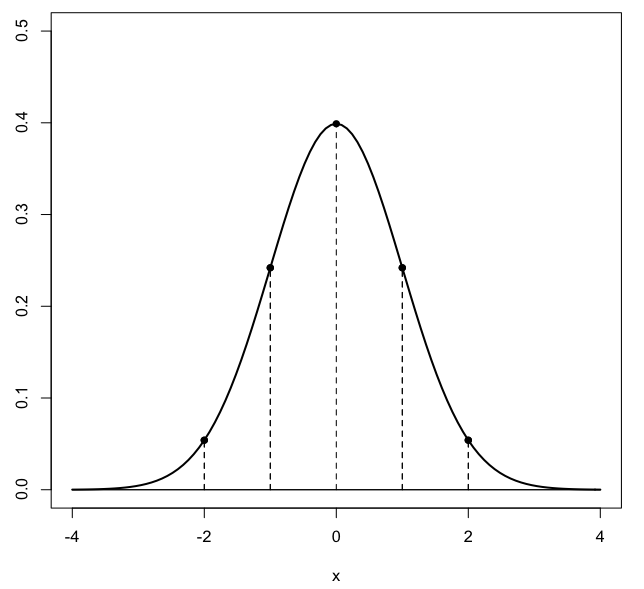
\includegraphics [scale=0.4] {gauss3.png} \end{center}

\title{Calculations}
\date{}

\begin{document}
\maketitle
\Large
Calculate Gregory formulas for perimeter and area of inscribed and circumscribed polygons for several rounds, preserving square roots.

\section*{perimeter}
recurrence:
\[ P' = \frac{2pP}{p + P} \ \ \ \ p' = \sqrt{pP'} \]
initialization:
\[ p = 2 \sqrt{2} \ \ \ \ P = 4 \]
\subsection*{round 1}
\[ P' = \frac{2 \cdot 2 \sqrt{2} \cdot 4}{2 \sqrt{2} + 4} =   \frac{2 \cdot 2 \sqrt{2} \cdot 4}{2 \sqrt{2}(1 + \sqrt{2})} = \frac{8}{1 + \sqrt{2}} \]
\[ p' = \sqrt{2 \sqrt{2} \cdot \frac{8}{1 + \sqrt{2}}} = 4 \sqrt{\frac{1}{1 + 1/\sqrt{2}}}  \]
\subsection*{round 2}
\[ P' = \]

\section*{area}

initialization:
\[ a = 2 \ \ \ \ A = 4 \]
recurrence:
\[ a' =  \sqrt{aA} \ \ \ \  A' = \frac{2a'A}{a' + A} \]


\end{document}